\subsection{Combustível GLP}
O uso de combustível GLP foi investigado no processo de aspersão a partir de
corpos de prova metálicos. A análise de desempenho é medida por ensaios de
adesão, metalografia e microdureza. Os elementos do teste são: pó de carboneto
de tungstênio com matriz de cobalto e cromo, GLP e oxigênio como gases da combustão, nitrogênio para
arraste do pó, ar comprimido e água para refrigeração da pistola, e uma pistola
de metalização Diamond Jet modelo DJ2700 (sulzer com refrigeração híbrida). O
equipamento de metalização utilizado para realização do processo de aspersão
produz a chama para a fusão do pó metálico a partir da combustão do
propano. Neste estudo foram realizados testes prévios utilizando-se o GLP como
gás combustível a fim de encontrar os parâmetros ideais de funcionamento do
equipamento para a deposição de um revestimento sem perda de características
técnicas. 

Os resultados foram comparados com os critérios pré-definidos pelo fabricante
da matéria prima e outros testes utilizando propano como
combustível. Nessa perspectiva, não houve perda de características técnicas do
revestimento a partir do uso do GLP como combustível. A importância desse teste
está relacionada com a facilidade de fornecimento de GLP em relação ao propano,
pois como se trata de uma solução abrangente e as usinas hidrelétricas
situam-se muitas vezes em locais ermos com baixas opções de fornecimento de
insumos. A distinção básica entre o GLP e o propano trata-se de que o GLP é uma
mistura de propano e butano e, além disso, possui custo reduzido (~ R\$ 5,00/kg)
de fornecimento em relação ao propano (~R\$16,00/kg). Deve ser feito uma
observação para utilização do GLP em locais frios, pois a sua temperatura de
vaporização é mais elevada tornando a vazão de fornecimento instável. Esse
problema não se aplica, porém, para a região de Porto Velho – RO onde se
encontra a UHE Jirau. A Fig.~\ref{fig:adequacao3} apresenta uma imagem do
ensaio de metalografia realizado em amostras de revestimento aspergido com GLP juntamente
com os resultados dos ensaios citados anteriormente.

\begin{figure}
	\centering
	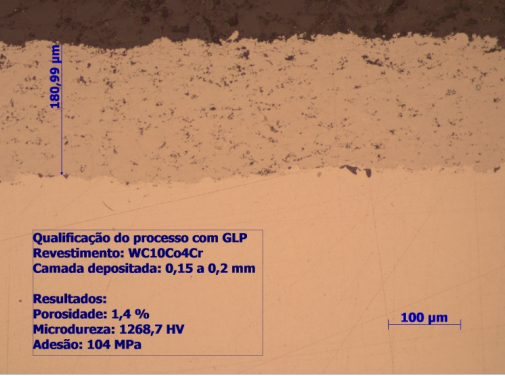
\includegraphics[width=1\columnwidth]{method/figs/adequacao/adequacao3.png}
    \caption{Propriedades do revestimento de Carboneto de Tungstênio-Cobalto-Cromo via HVOF com combustível GLP.}
    \label{fig:adequacao3}
\end{figure}